\renewcommand{\thesection}{\arabic{section}}
\titleformat{\section}{\normalfont\large\bfseries}{\thesection. pielikums.}{1em}{}

\section{Ar rāpuļa palīdzību izgūta raksta piemērs}
\noindent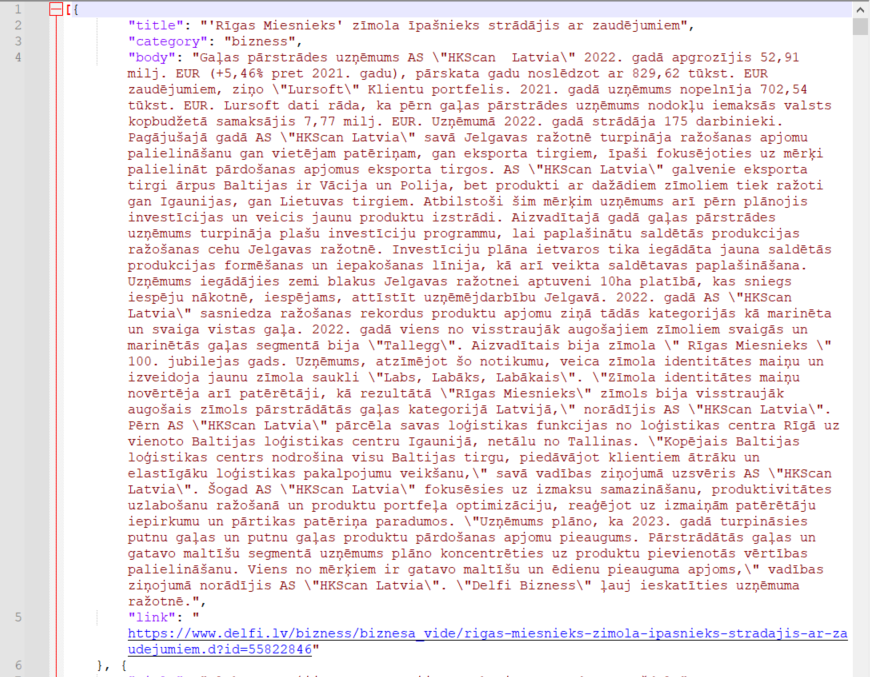
\includegraphics[width=\textwidth]{raksta_piemers}
\addtocounter{nofappendices}{1}
\label{appendix:raksta_piemers}

\section{Klasificējamo kategoriju rakstu garumi}
\noindent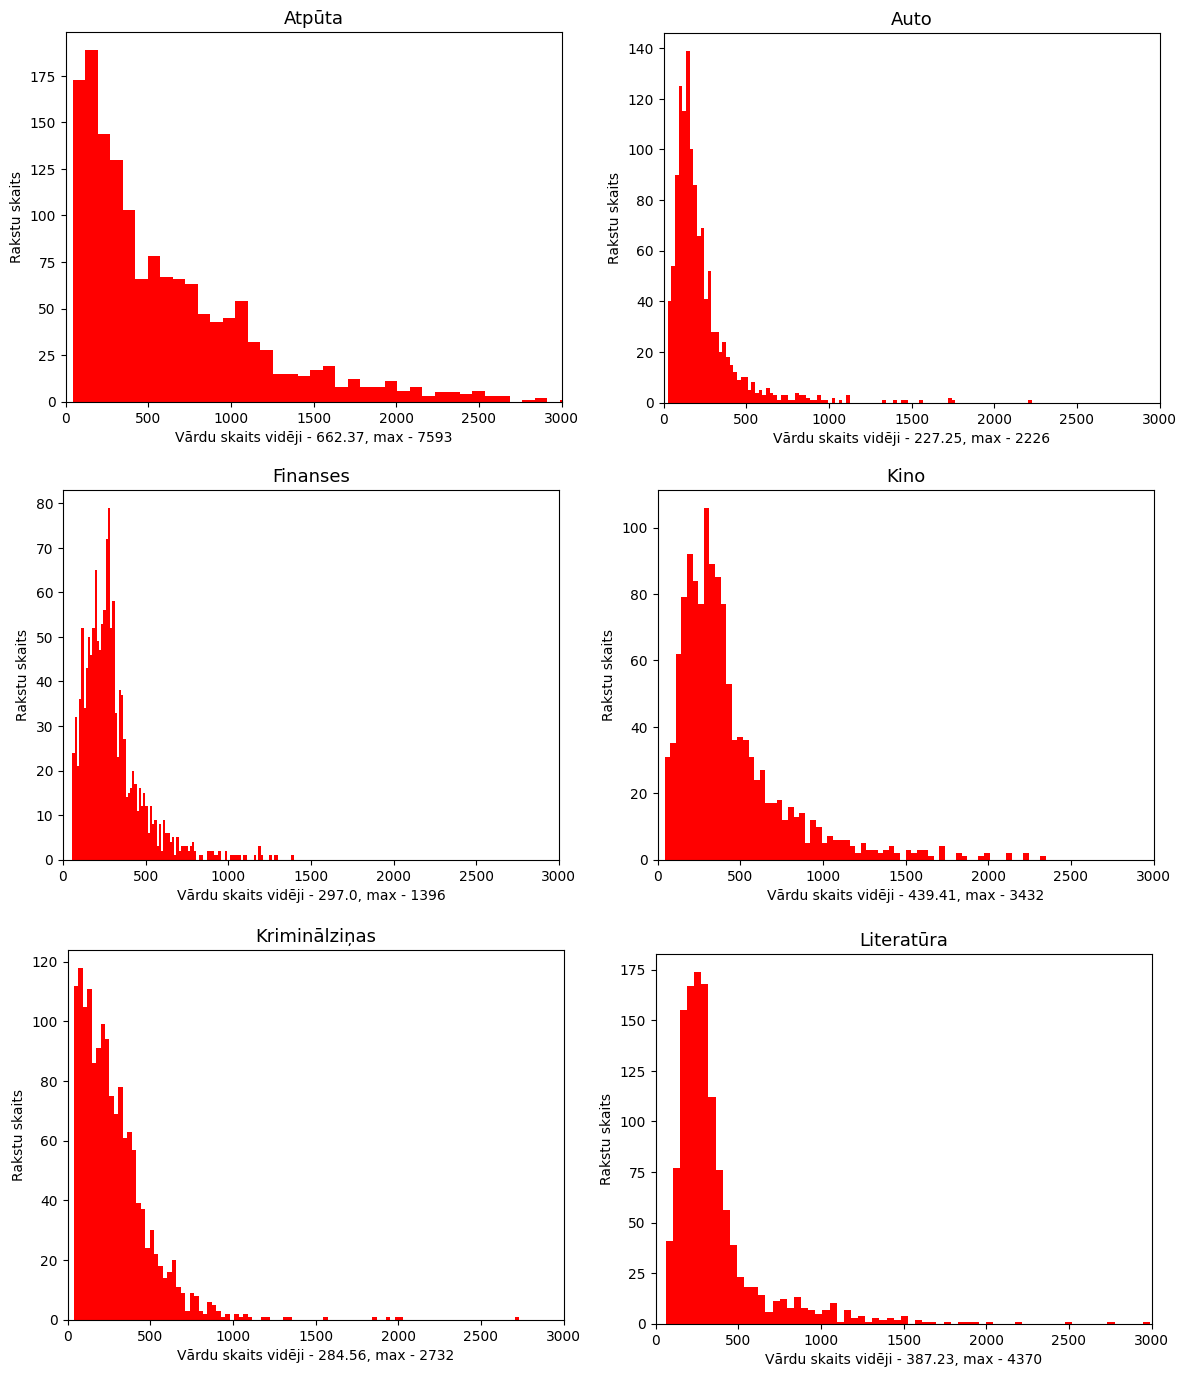
\includegraphics[width=\textwidth]{kategorijas_wc}
\addtocounter{nofappendices}{1}
\label{appendix:kategorijas_wc}